\documentclass[aps,prb,onecolumn,notitlepage,showpacs,floatfix,superscriptaddress]{revtex4-1}
\usepackage{dcolumn}
\usepackage{tabularx}
\usepackage{bm}
\usepackage{soul}
\usepackage{amsmath,amssymb,graphicx}
\usepackage[colorlinks=true,citecolor=blue,urlcolor=blue,linkcolor=blue]{hyperref}
\usepackage{environ}

\NewEnviron{eqnsplit}{%
\begin{equation}
\begin{split}
  \BODY
\end{split}
\end{equation}
}

\newcommand{\mrm}[1]{\mathrm{#1}}
\newcommand{\ang}{\mathrm{\AA}}

\bibliographystyle{apsrev4-1}

%%%%%%%%%%%%%%%%%%%%%%%%%%%%%%%%%%%%%%%%%%%%%%%%
\begin{document}
\title{Nuclear Magnetic Resonance (NMR)}

\author{Avinash Rustagi}
\email{arustag@ncsu.edu}
\affiliation{Department of Physics, North Carolina State University, Raleigh, NC 27695}
%
\date{\today}
%%%%%%%%%%%%%%%%%%%%%%%%%%%%%%%%%%%%%%%%%%%%%%%%

\maketitle
Nuclear Magnetic Resonance (NMR) is a powerful experimental measurement techniques useful in characterizing compounds with magnetic constituents. The physics of NMR is based on the nuclear magnetic moment of the nuclei which has an angular momentum. The magnetic moment ${\bm \mu}$ and the angular momentum ${\bm J}$ are related by
\begin{equation}
{\bm \mu} = \gamma {\bm J}
\end{equation} 
where $\gamma$ is the gyromagetic ratio. In presence of a magnetic field ${\bm B}=B_0 \hat{z}$, the magnetic energy is
\begin{equation}
U=-{\bm \mu} \cdot {\bm B} = - \mu_z B_0 = -\gamma J_z B_0
\end{equation}
\begin{figure}[hbtp]
\centering
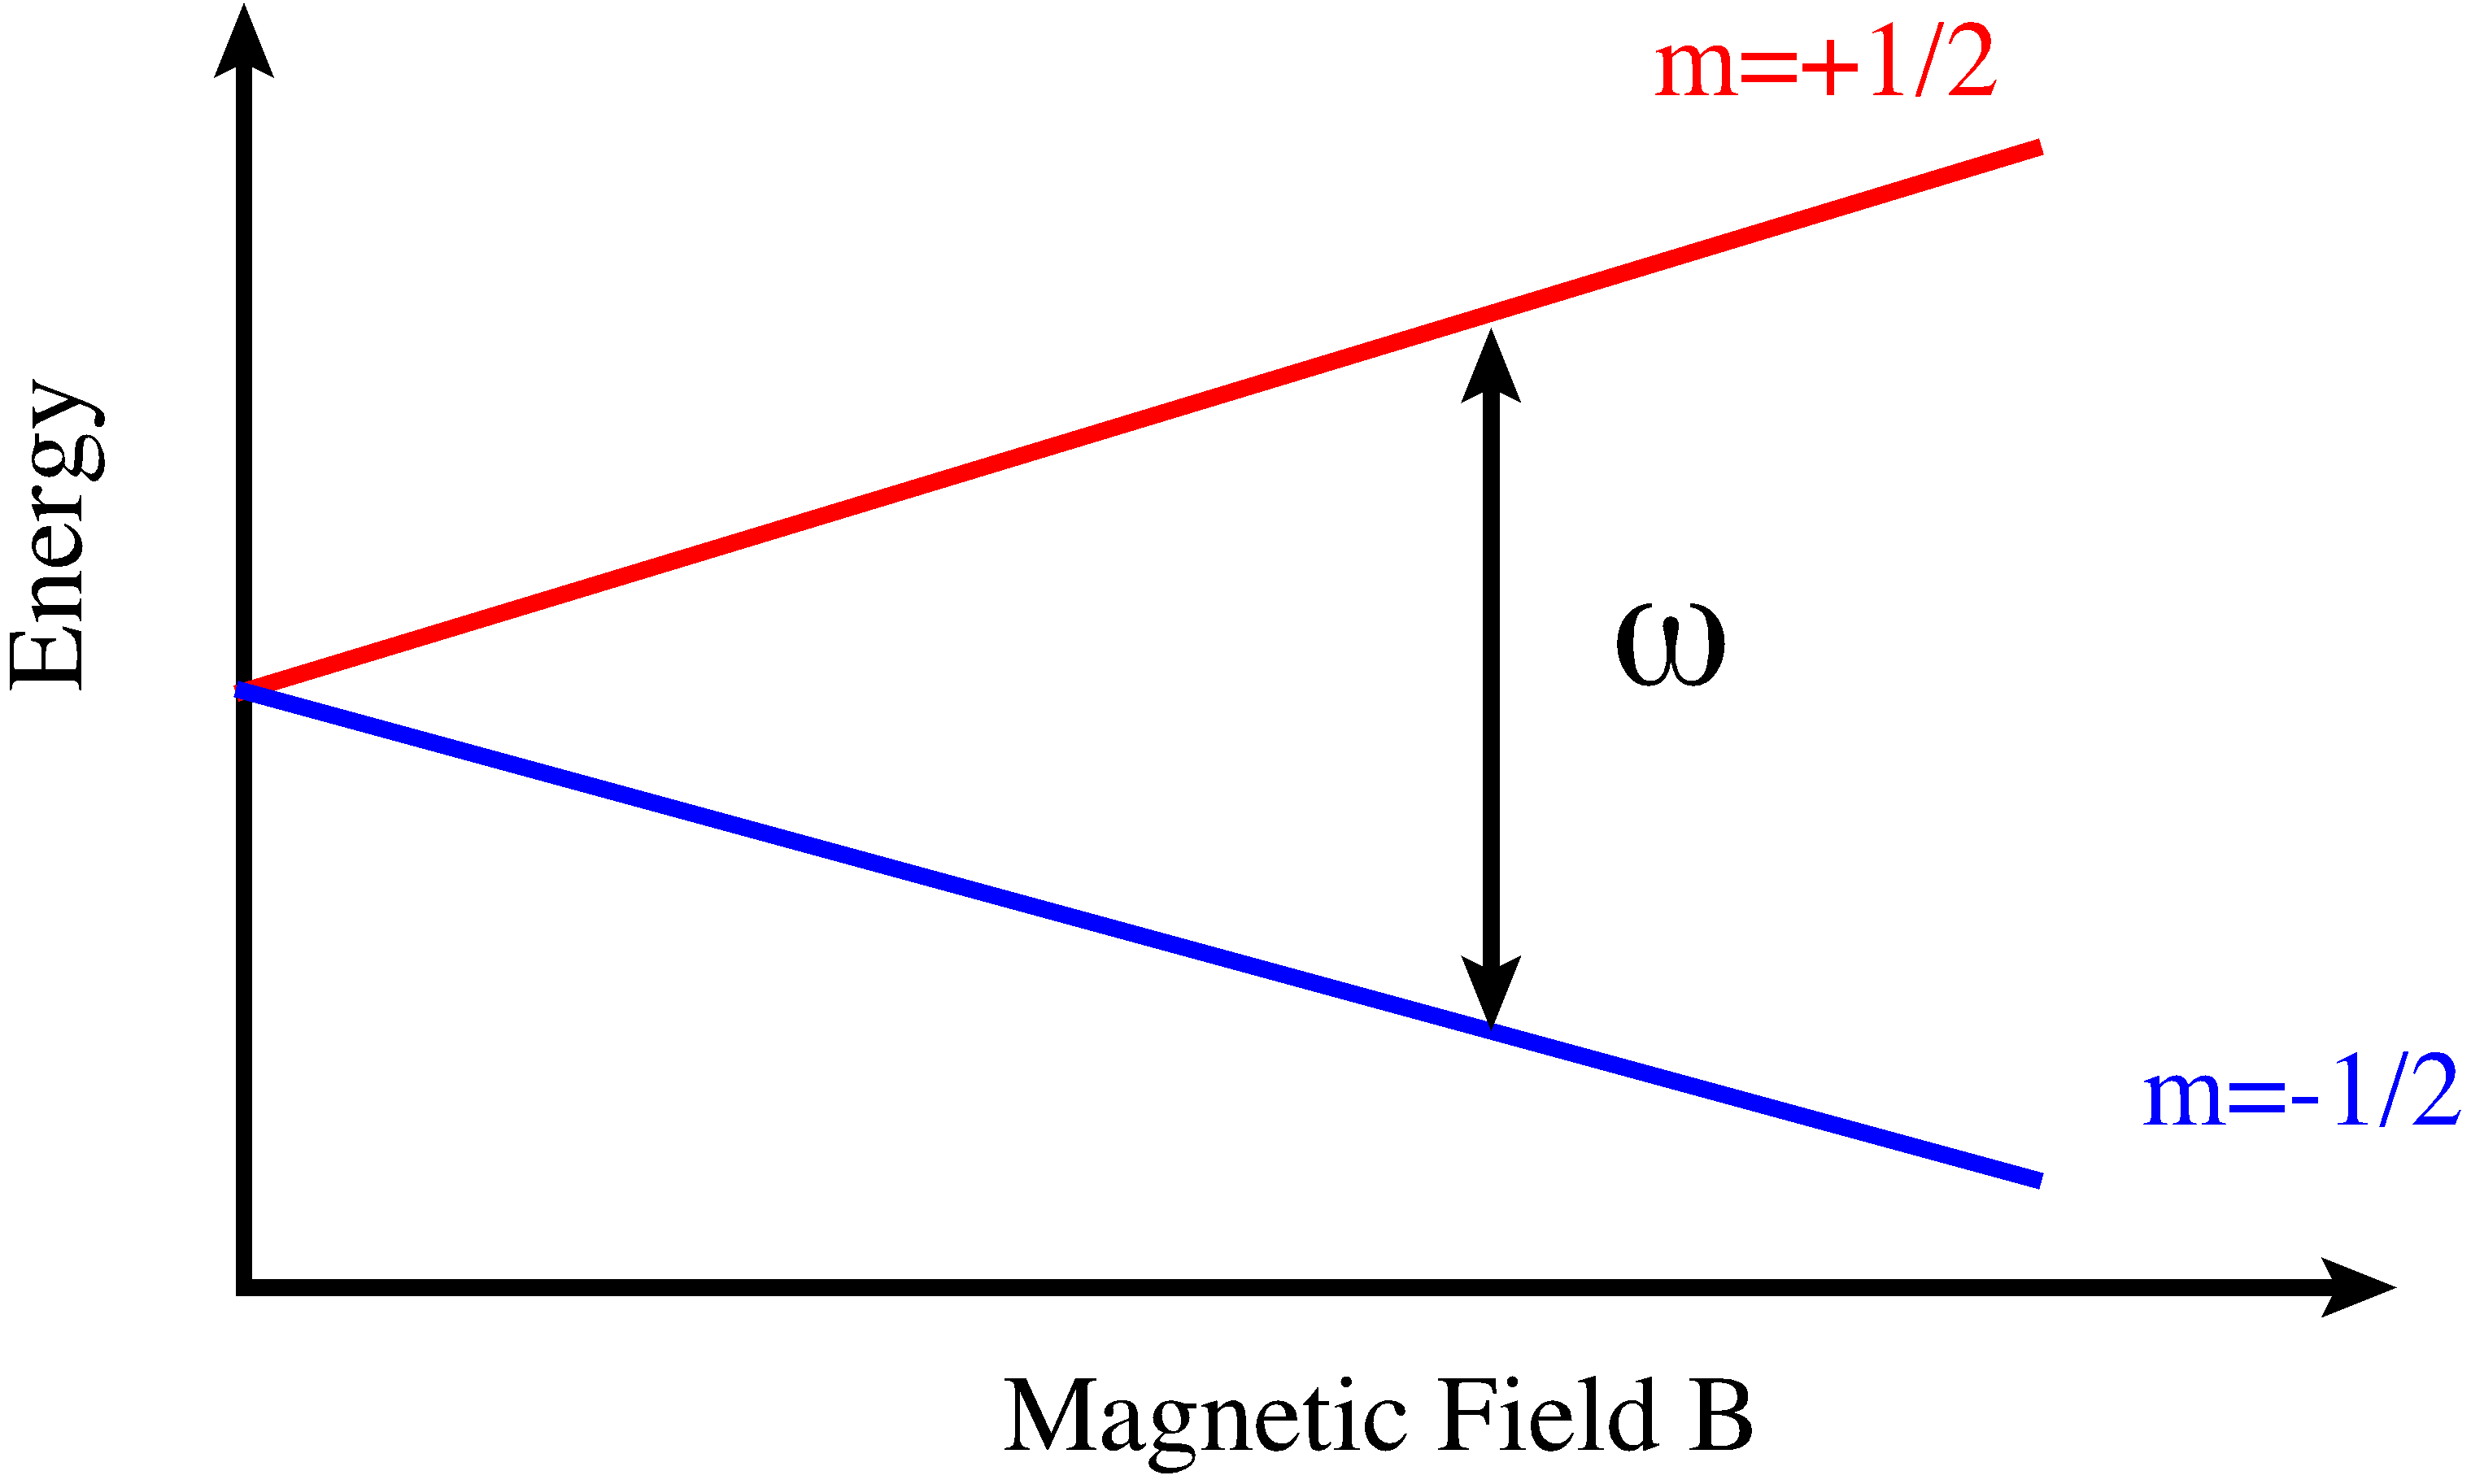
\includegraphics[scale=0.06]{Zeeman.png}
\caption{Zeeman Splitting in magnetic field.}
\end{figure}
Considering the simplest case of a proton that has spin 1/2, $J_z = m \hbar$ where $m= \pm 1/2$. This means that the magnetic energy is minimized when the spin aligns with the magnetic field
\begin{equation}
U= -\gamma m \hbar B_0
\end{equation}
The energy difference between the aligned and anti-aligned configuration is expressed in terms of a frequency
\begin{equation}
\Delta U = \hbar \omega_0 = \gamma \hbar B_0 \Rightarrow \omega_0 = \gamma B_0
\end{equation}
The frequency $\omega_0$ is the resonance frequency when energy can be absorbed by an aligned spin to become anti-aligned. In thermal equilibrium with no magnetic field, the number of aligned $N_1$ and anti-aligned $N_2$ spin are equal. However, in presence of a magnetic field
\begin{equation}
\dfrac{N_2}{N_1} = \exp\left( -\dfrac{\Delta U}{K_B T}\right)
\end{equation}
with magnetization ${\bm M} = (N_! -N_2) {\bm \mu}$, since more spins aligned with the field to lower the magnetic energy. It is worth emphasizing that the spins do not align in the field direction instantaneously. The z-component of magnetization $M_z$ grows exponentially with time and satisfies 
\begin{equation}
\dfrac{dM_z}{dt} = -\dfrac{M_z -M_0}{T_1}
\end{equation}
where $M_0$ is the thermal equilibrium magnetization
\begin{equation}
M_0 = N \mu \tanh \left( \dfrac{\mu B_0}{k_B T} \right) \qquad N=N_1 +N_2
\end{equation}
The time constant $T_1$ is known as the `spin-lattice' relaxation time. This is so because the aligning of spins happens when individual spin lose energy to the surroundings. The surrounding that absorbs this energy is referred to as the `lattice'. Thus the time constant $T_1$ is the characteristic time of this energy flow from the spins to the lattice.

Magnetic moment in presence of a magnetic field experiences a torque. The moment precesses about the field. Only the net magnetization in the field direction is non-zero $=M_0$. The other components add up to zero when accounted for all the magnetic moments. In classical mechanics
\begin{equation}
{\bm T} = {\bm \mu} \times {\bm B} \qquad \dfrac{1}{\gamma} \dfrac{d {\bm \mu}}{dt} = {\bm \mu} \times {\bm B} 
\end{equation}
The precessional frequency is $\omega_0$. If the components of magnetic moments are added for all the protons $\sum \mu_z = M_0$, $\sum \mu_x = \mu_y= 0$. This means that there is no phase relationship between the x-y components of magnetic moment of the different protons. The torque equation can be generalized to an equation for the magnetization
\begin{equation}
 \dfrac{d {\bm M}}{dt} =\gamma {\bm M} \times {\bm B} 
\end{equation}
It is possible to create a transverse magnetization by application of a radio frequency pulsed magnetic field. Suppose in addition to the constant magnetic field $B_0 \hat{z}$, we apply a rotating (circularly polarized) magnetic field $B_1 \left( \cos \omega t \,\hat{x} + \sin \omega t \, \hat{y}\right)$ in the x-y plane. This situation can best be applied by moving to a rotating frame $(\hat{x},\hat{y},\hat{z}) \rightarrow (\hat{x}^*,\hat{y}^*,\hat{z}^*)$. To analyze this, we need to figure out the magnetic field seen in the rotating frame. If we move to a rotating frame that rotates with frequency $\omega$, the moving observer sees a constant field $B_1$ along the x$^*$-direction. 

If we had a constant field in the z$^*$-direction, we know that the magnetization precesses about the field with Larmor frequency. If we are in a frame that rotates with Larmor frequency, the magnetization will appear stationary to us. This can only happen if the torque acting the magnetization is zero. Hence the net magnetic field is zero, which implies that in the rotating frame $ = (B_0 - \omega_0 /\gamma)\hat{z}^*$. 

\begin{figure}[hbtp]
\centering
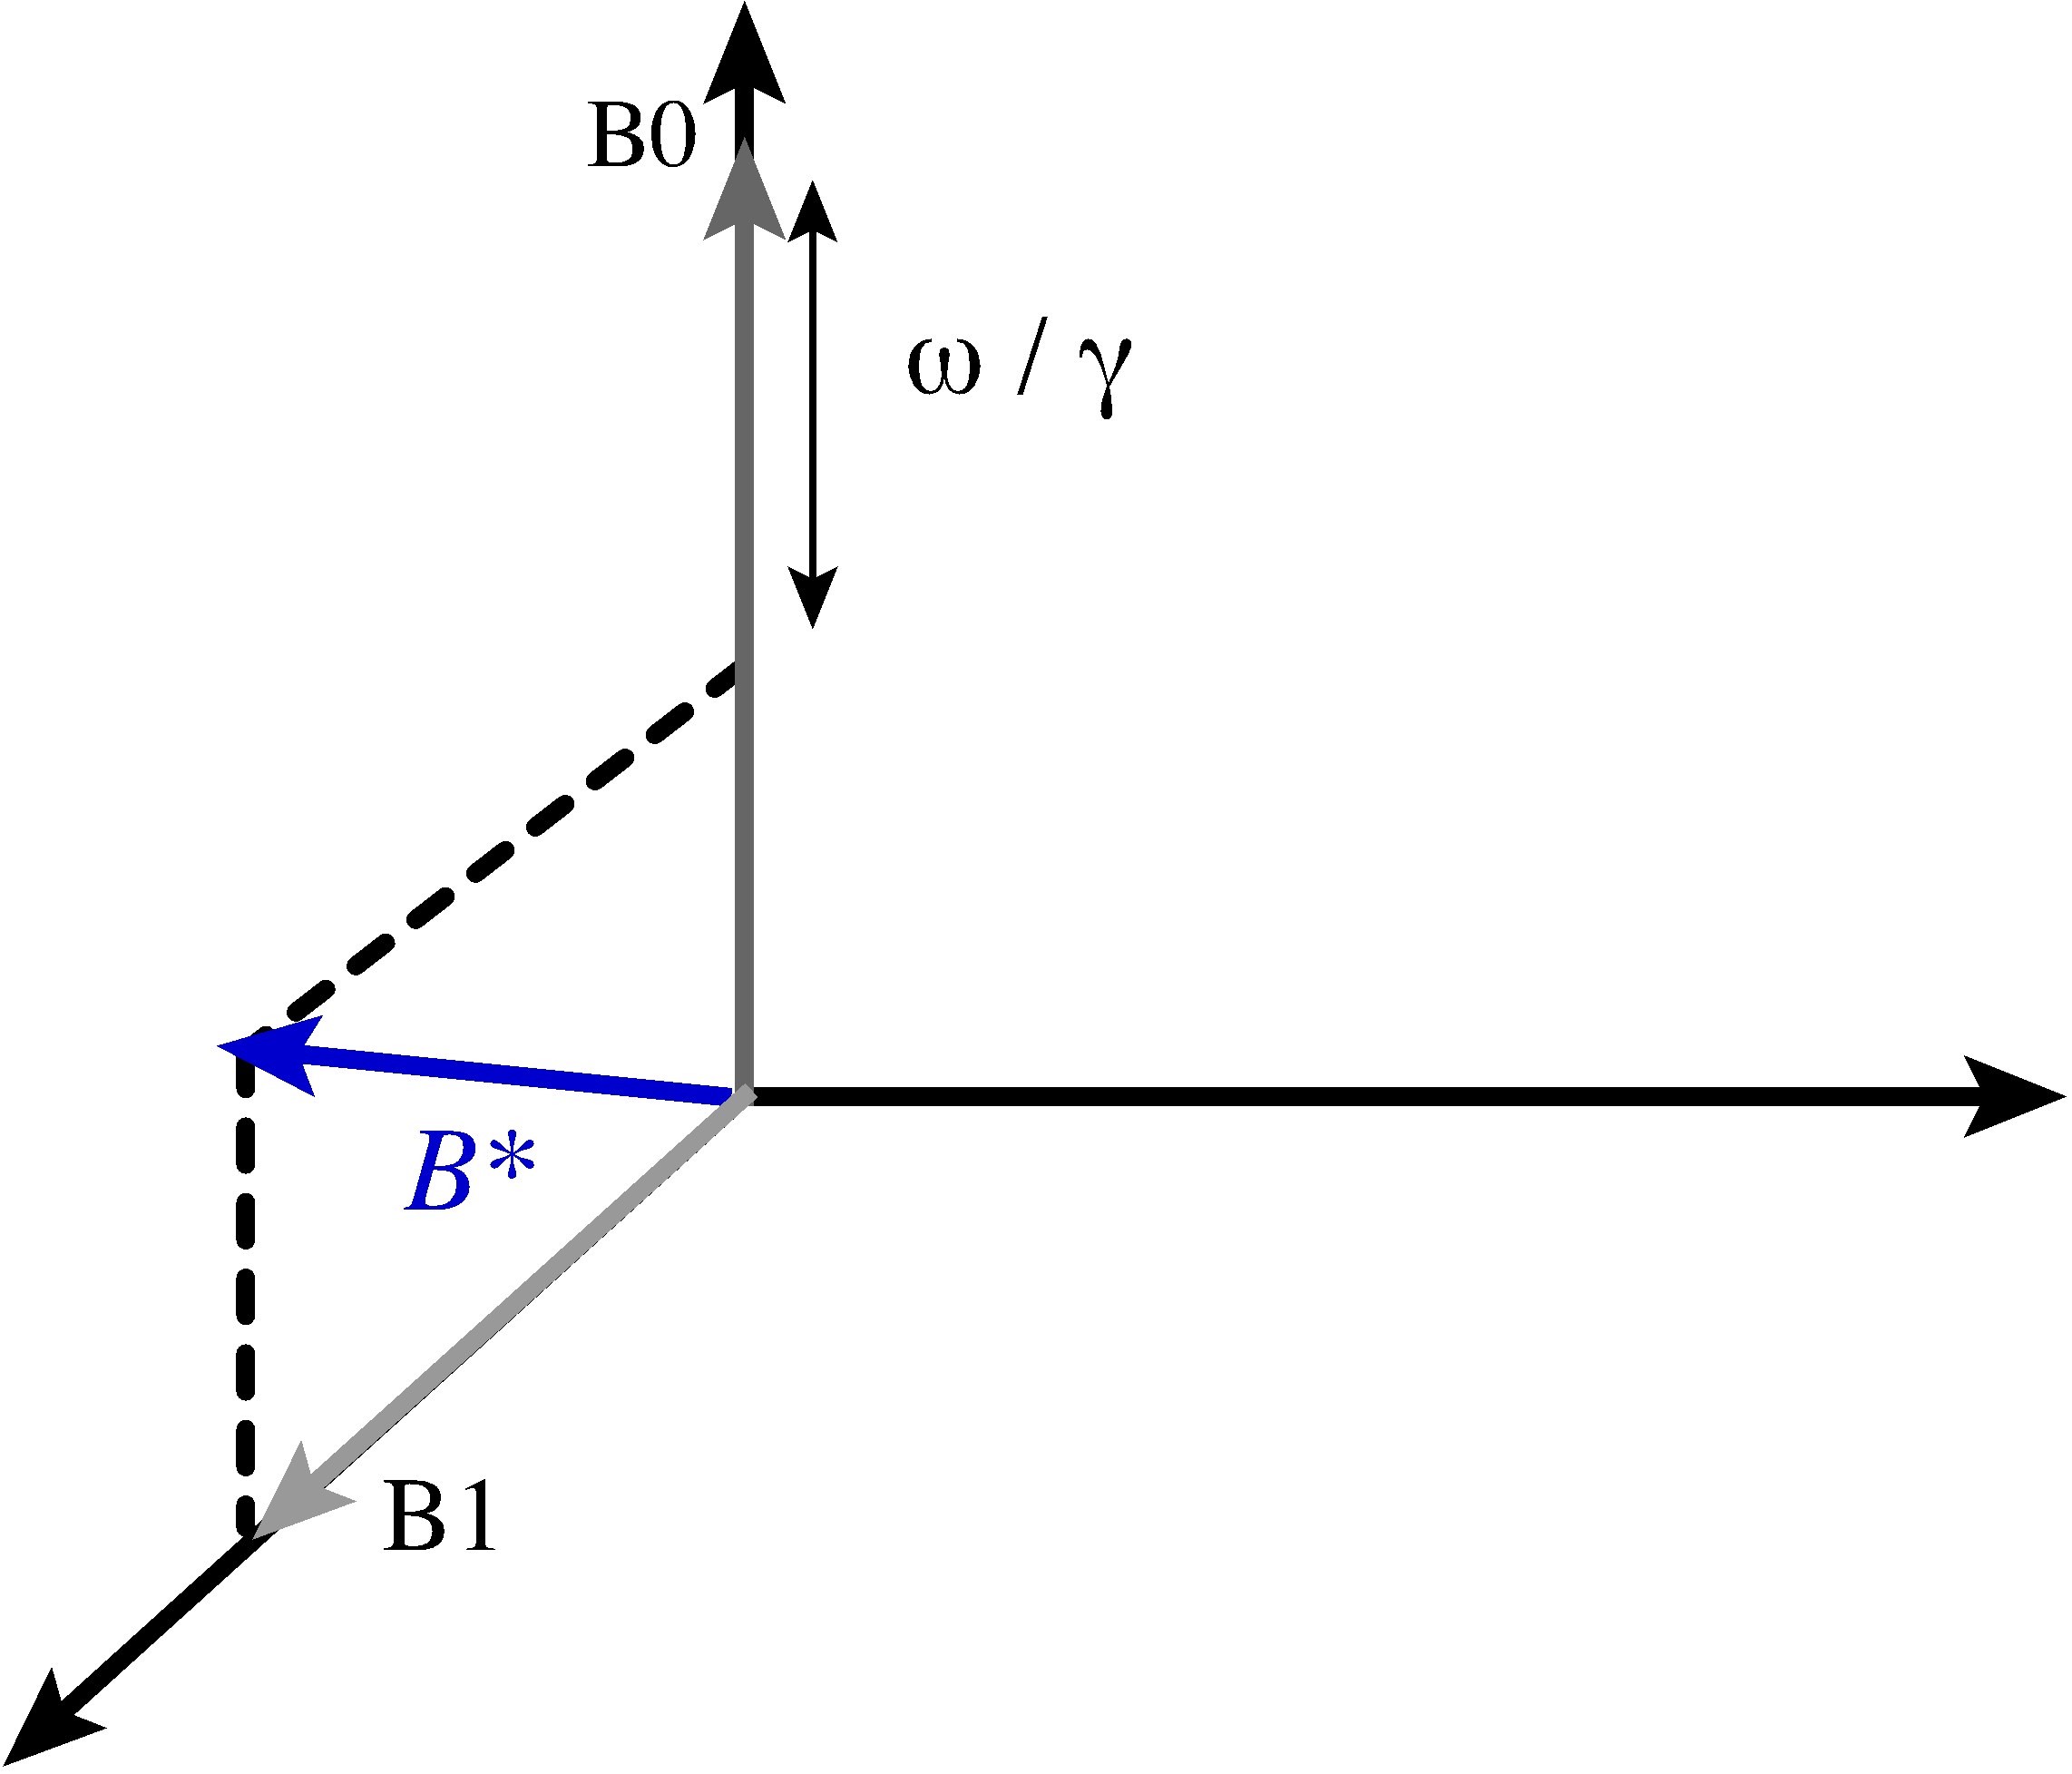
\includegraphics[scale=0.06]{B_in_RF.png} 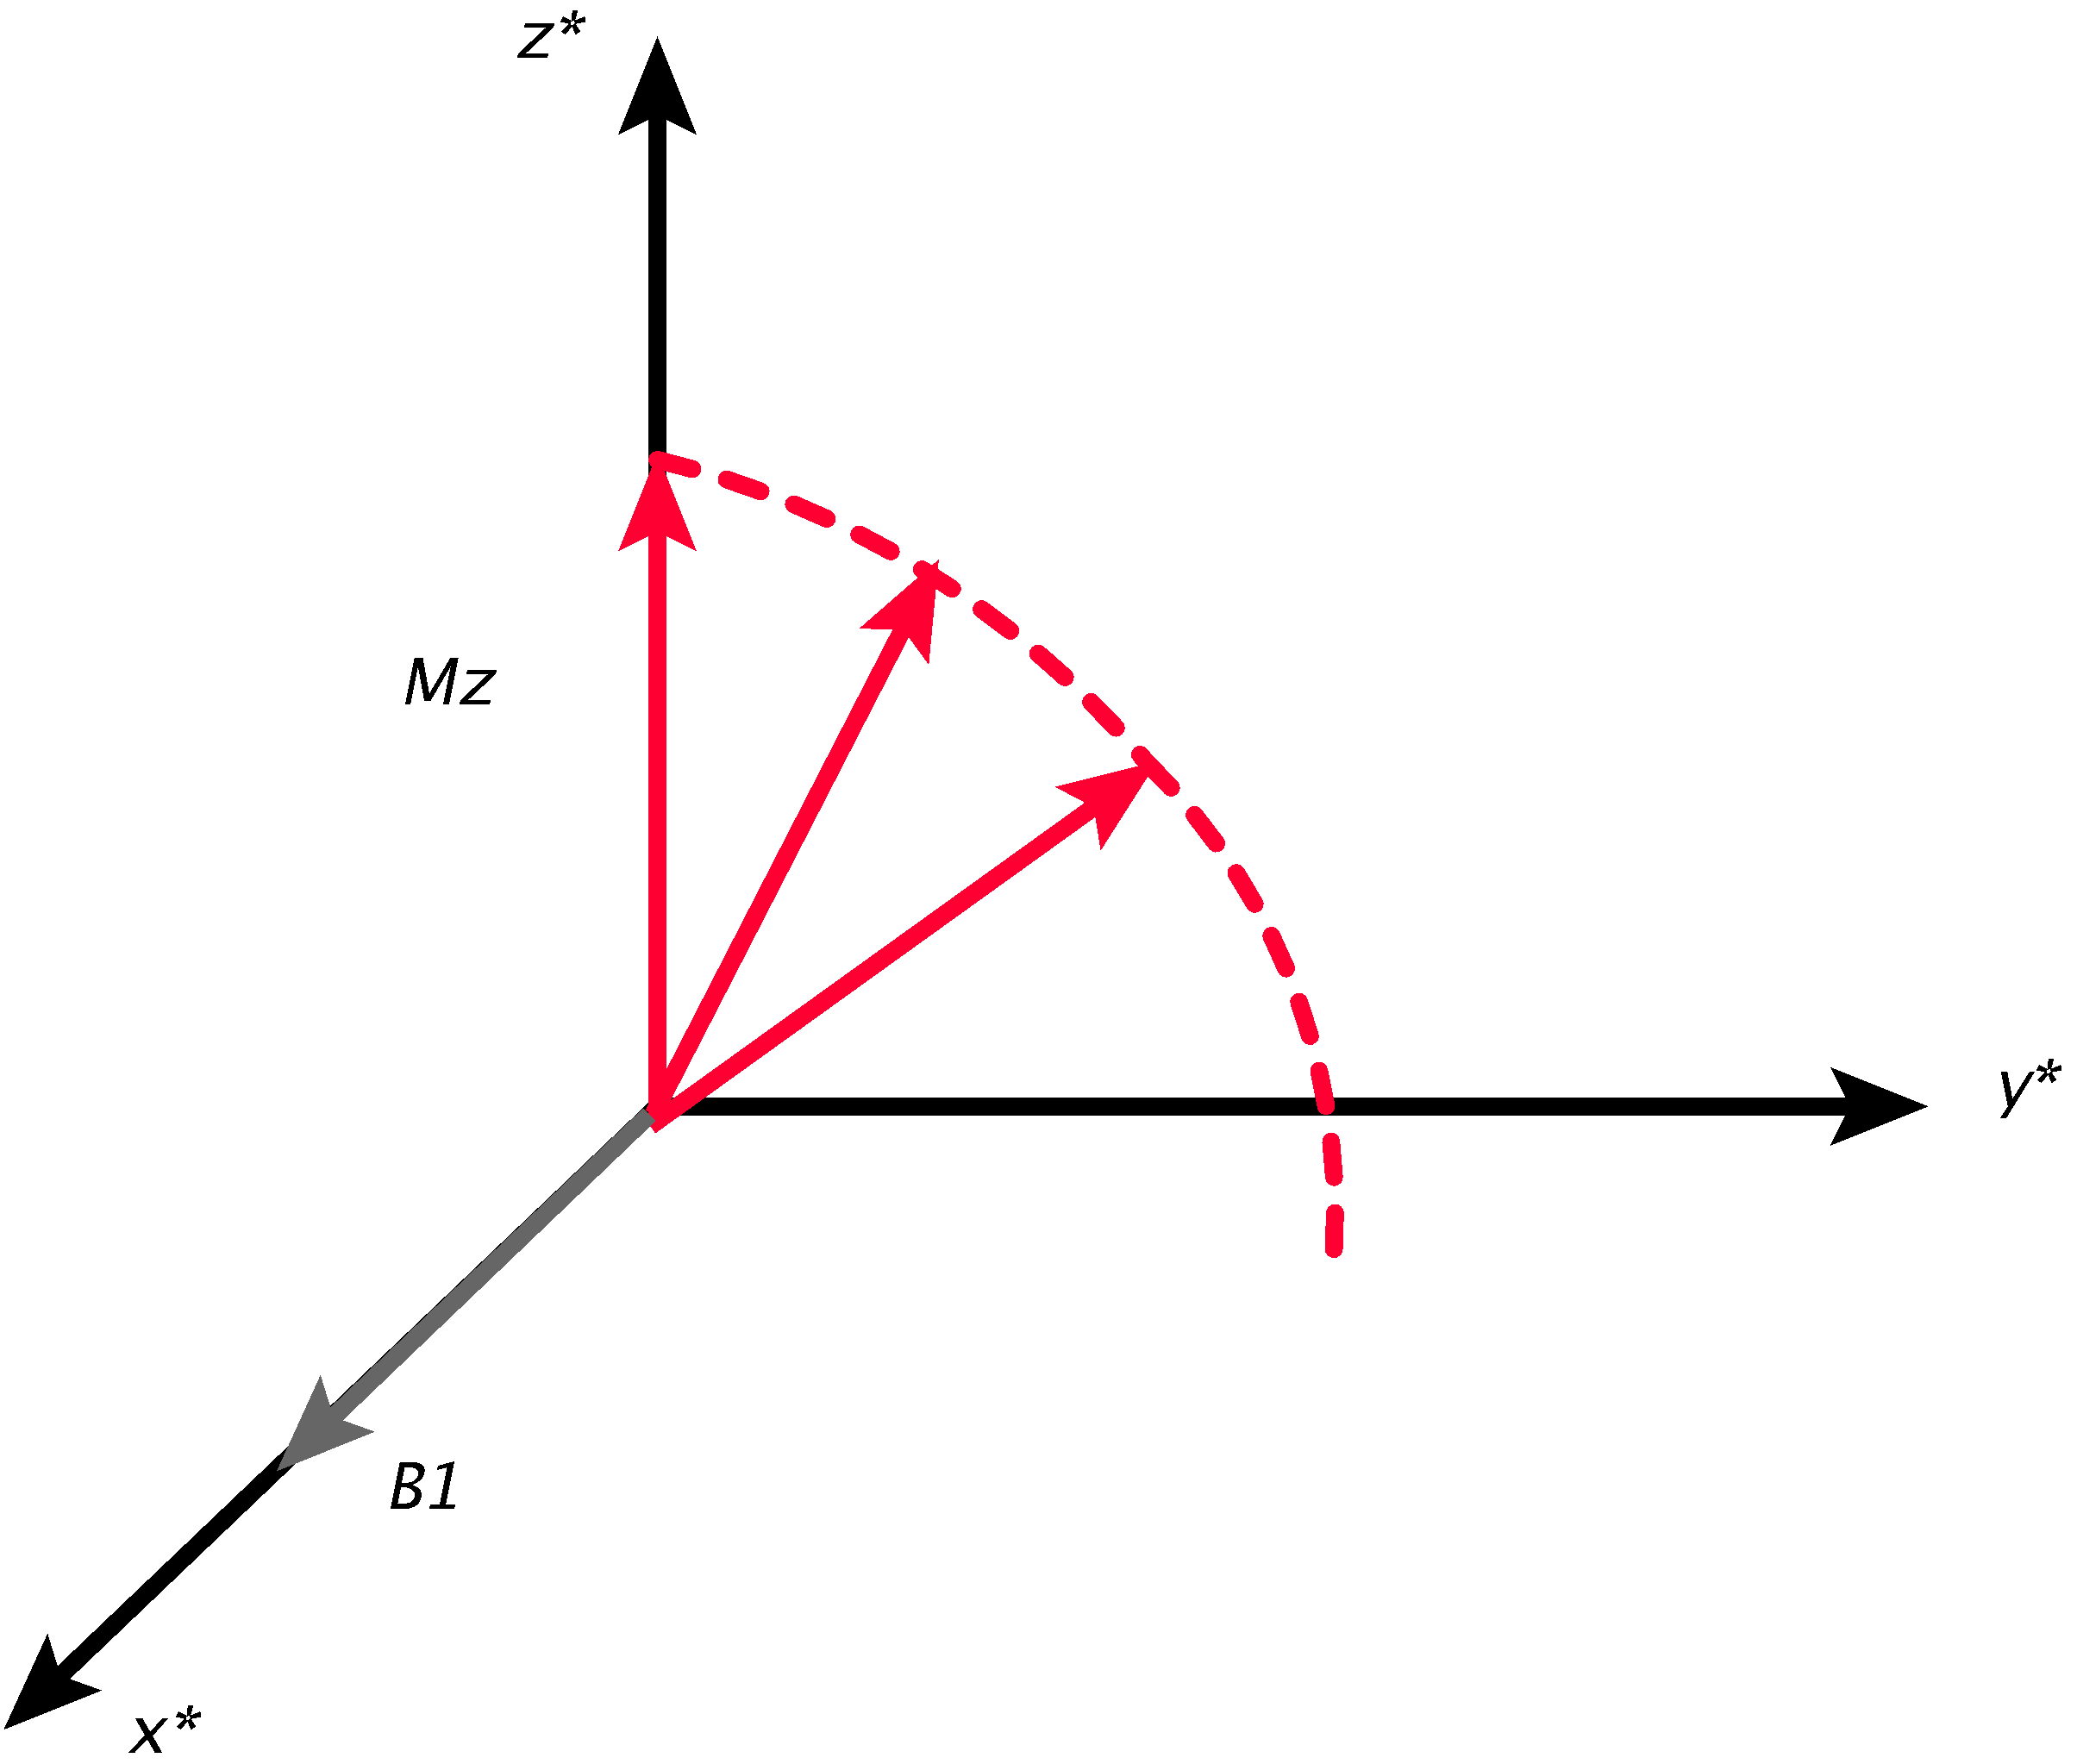
\includegraphics[scale=0.06]{pulsed.png}
\caption{Effective Field in the rotating frame.}
\end{figure}

Thus for a frame rotating with frequency $\omega$, the magnetic field in the z-direction would be $ = (B_0 - \omega /\gamma)\hat{z}^*$. Thus the net field in the rotated frame is
\begin{equation}
{\bm B}^* = (B_0 - \omega /\gamma)\hat{z}^* + B_1 \, \hat{x}^*
\end{equation}
In the rotating frame
\begin{equation}
 \dfrac{d {\bm M}^*}{dt} =\gamma {\bm M}^* \times {\bm B}^* 
\end{equation}
Thus if we choose $\omega=\omega_0$, then we only have a constant field in the x-direction. Thus the net magnetization $M_z^*$ now precesses about this field. If we now turn off the $B_1$ field when the magnetization is in the x-y plane. We can also turn off the $B_1$ field when the magnetization is in the -z direction, These are called
\begin{equation}
\begin{split}
&90^o \,\,\text{or} \,\, \pi/2 \,\, \text{pulse} \Rightarrow M_z^* \rightarrow M_y^* \\
&180^o \,\,\text{or} \,\, \pi \,\, \text{pulse} \Rightarrow M_z^* \rightarrow -M_z^* \\
&360^o \,\,\text{or} \,\, 2\pi \,\, \text{pulse} \Rightarrow M_z^* \rightarrow M_z^* 
\end{split}
\end{equation}
The experiment is performed in the laboratory frame where the magnetization not only precesses about ${\bm B_1}$ but also about $\hat{z}$. Since we are dealing with pulsed ${\bm B}_1$, there are signatures after this RF field pulse is over. Suppose we have a 90$^o$ pulse, the magnetization will be rotated into the x*-y* plane, which will subsequently precess about the z*-direction. The x*-y* magnetization will decay exponentially
\begin{equation}
\dfrac{d M_x^*}{dt} =-\dfrac{M_x^*}{T_2} \qquad \dfrac{d M_y^*}{dt} =-\dfrac{M_y^*}{T_2}
\end{equation}
$T_2$ is the spin-spin relaxation time. This can be understood since each proton produces a magnetic field which interacts with other protons. Each of the spins that are initially in phase after the 90$^o$ pulse will eventually dephase and the net x-y magnetization goes to zero. Thus a measurement of $T_2$ provides information of the distribution of local fields at the nuclei sites.

In the rotating frame with frequency $\omega$, the Bloch equation for the magnetization are
\begin{equation}
\begin{split}
\dfrac{d {\bm M}^*}{dt} =\gamma {\bm M}^* \times {\bm B}^* =  \gamma (B_0 - \omega/\gamma) {\bm M}^* \times \hat{z}^* + \gamma B_1 {\bm M}^* \times \hat{x}^* \\
\end{split}
\end{equation}
Including the relaxation times,
\begin{equation}
\begin{split}
\dfrac{d M_x^*}{dt} &=  (\omega_0 - \omega) M_y^* -\dfrac{M_x^*}{T_2} \\
\dfrac{d M_y^*}{dt} &=  -(\omega_0 - \omega) M_x^*+\gamma B_1 M_z^* -\dfrac{M_y^*}{T_2} \\
\dfrac{d M_z^*}{dt} &=  -\gamma B_1 M_y^* -\dfrac{M_z^*-M_0}{T_1} \\
\end{split}
\end{equation}
$M_z^*=M_z$ since we are rotating about the z-axis. The above set of equations can be solved. Looking at times when the pulsed $B_1$ field is over, we can set $B_1 =0$ and solve the equations in the rotating frame. Using transformations, we can obtain the magnetization in the laboratory frame.
\begin{equation}
\begin{split}
M_x^* &= M_x \cos \omega t - M_y \sin \omega t \\
M_y^* &= M_x \sin \omega t + M_y \cos \omega t \\
M_z^* &= M_z\\
\end{split}
\end{equation}

\begin{figure}[hbtp]
\centering
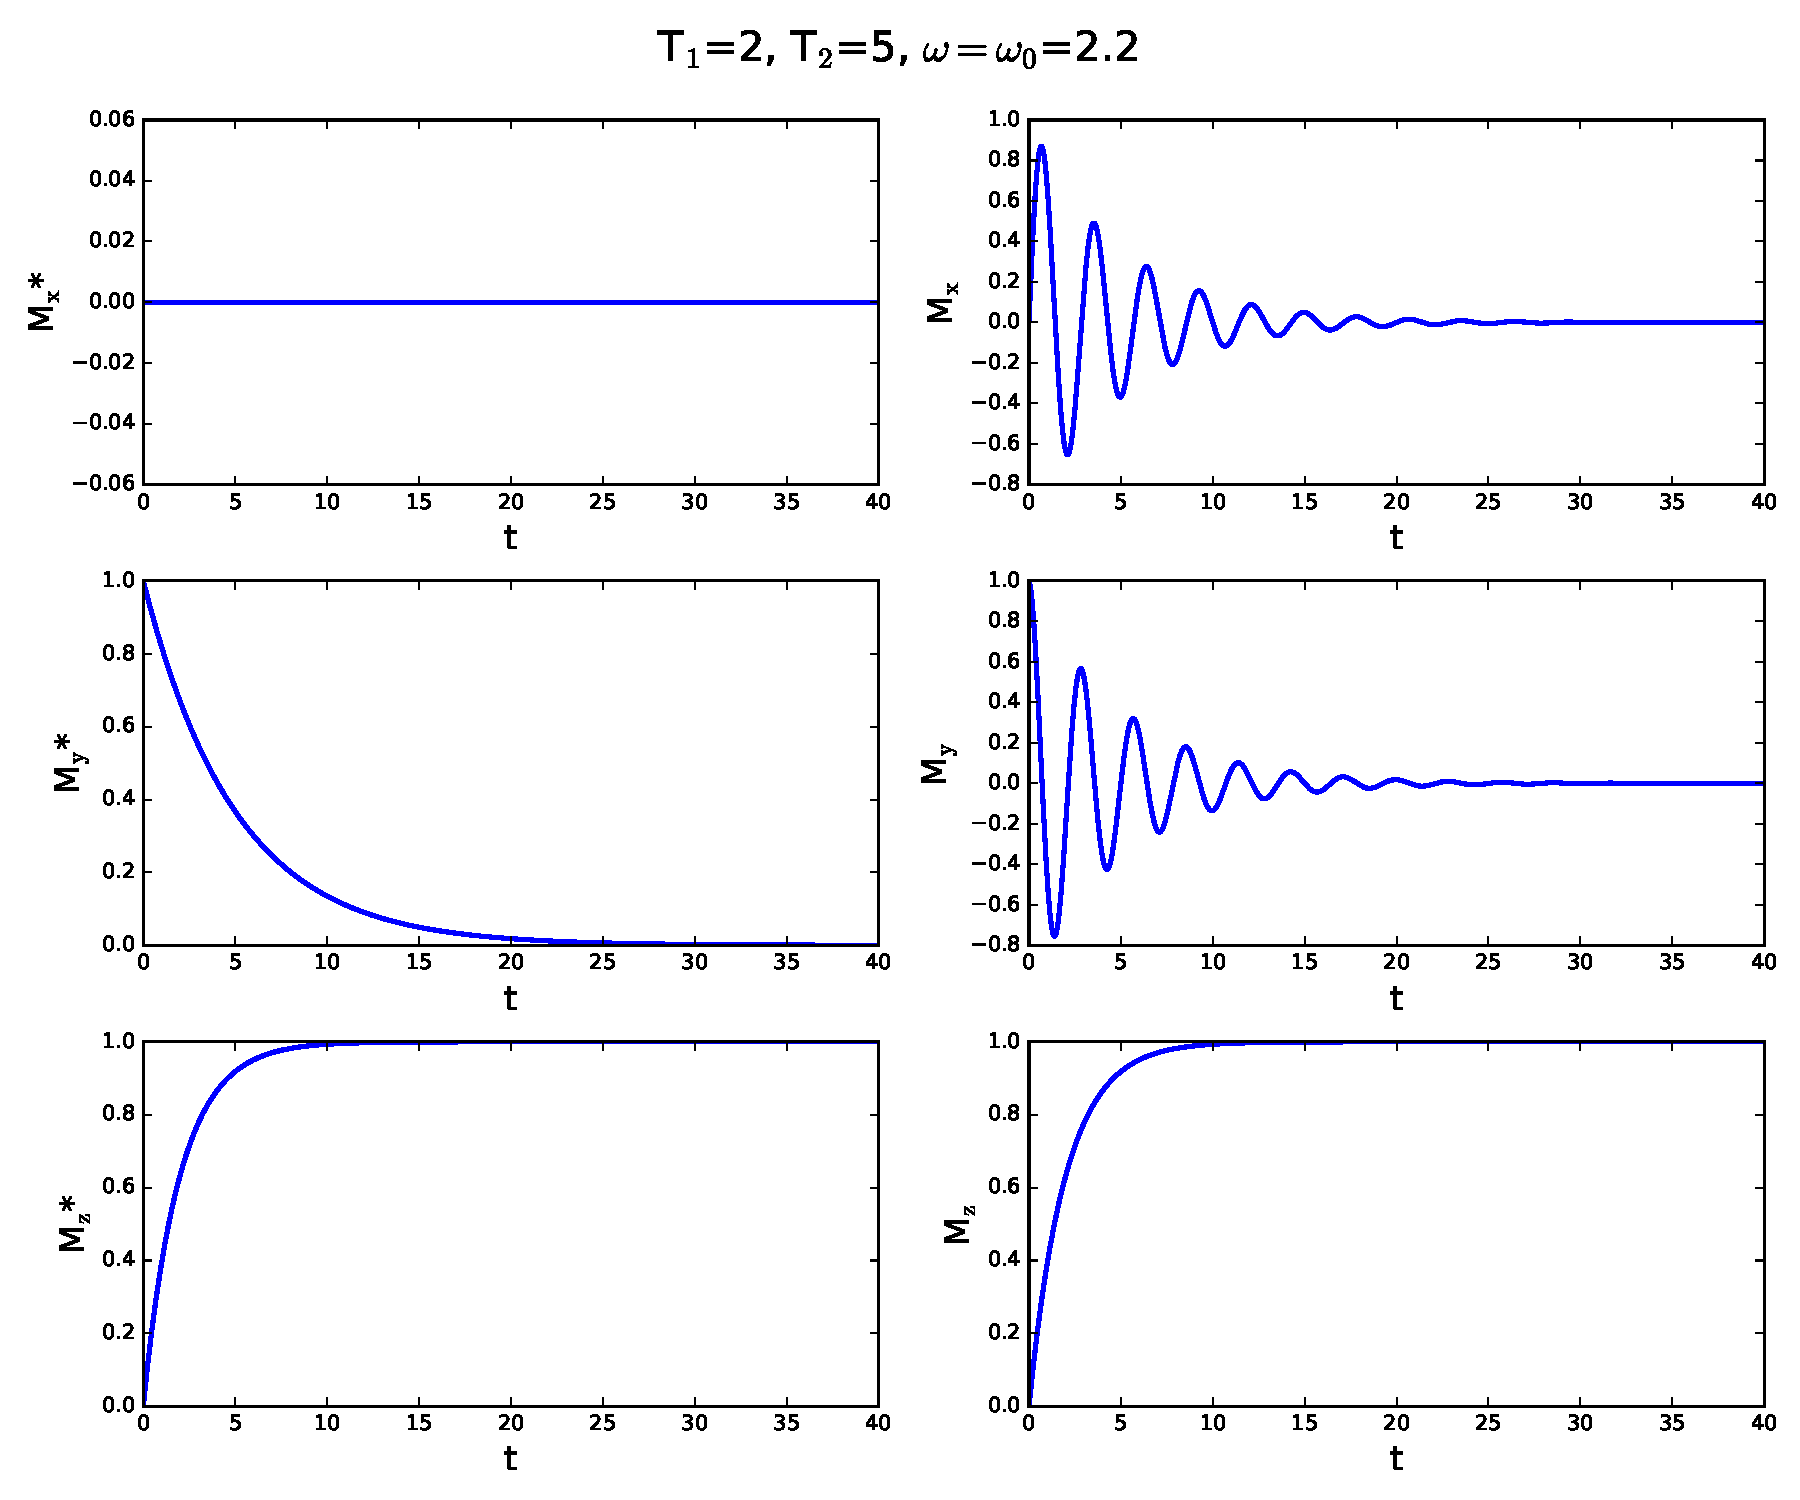
\includegraphics[scale=0.5]{RF_LF.pdf}
\caption{Time variation of the Magnetization components in the rotating and laboratory frame.}
\end{figure}


The NMR experiment involves applying a RF field in the x-y plane. The coil that generates this RF field also acts as a receiver for NMR signal. The rotating magnetization in the x-y plane generates a current picked up by the coil. The induced current in the coil oscillates with the frequency of the precessing spin. Thus different spins precessing with different Larmor frequencies contribute to the total induced current. The Fourier transform of the NMR signal/induced current shows these frequencies.
\end{document}